\documentclass{standalone}

\usepackage{tikz}
\usetikzlibrary{backgrounds, positioning, decorations.pathreplacing, calc, fit}
\usetikzlibrary{shapes}

\begin{document}

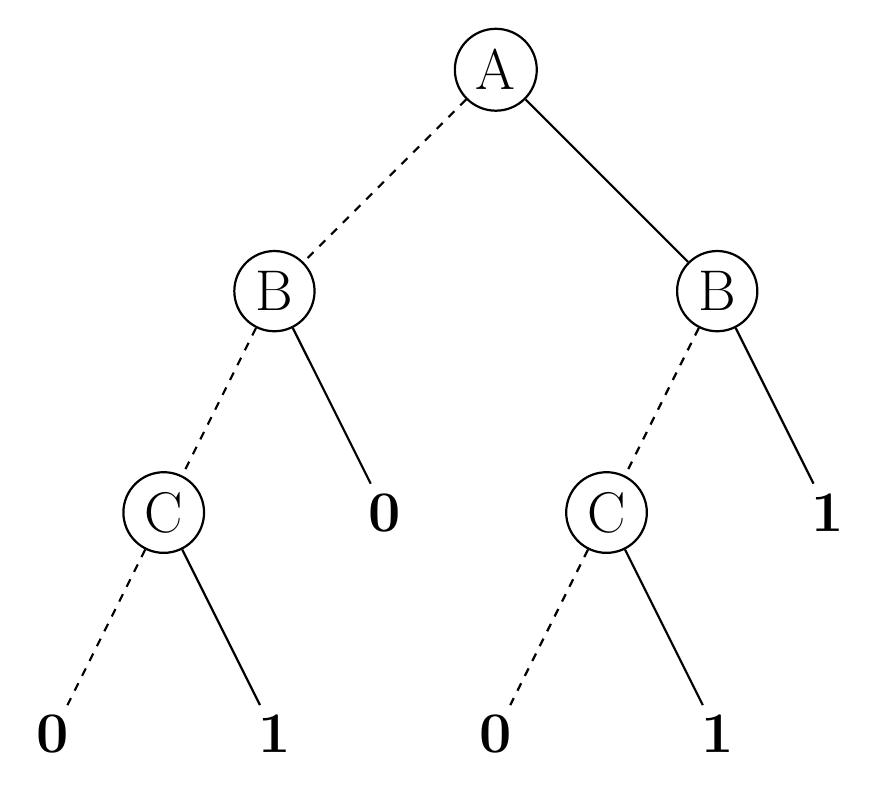
\begin{tikzpicture}[
    level 1/.style = { sibling distance = 16em, level distance = 8em },
    level 2/.style = { sibling distance = 8em, level distance = 8em }
]
    \tikzstyle{inner} = [draw, solid, circle, thick];

    \node[inner] at (0, 0) {\huge{A}}
    child[thick, dashed] {
        node[inner] {\huge{B}}
        child {
            node[inner] {\huge{C}}
            child[thick, dashed] { node {\textbf{\huge{0}}} }
            child[thick, solid] { node {\textbf{\huge{1}}} }
        }
        child[thick, solid] { node {\textbf{\huge{0}}} }
    }
    child[thick, solid] {
        node[inner] {\huge{B}}
        child[thick, dashed] {
            node[inner] {\huge{C}}
            child[thick, dashed] { node {\textbf{\huge{0}}} }
            child[thick, solid] { node {\textbf{\huge{1}}} }
        }
        child[thick, solid] { node {\textbf{\huge{1}}} }
    };
\end{tikzpicture}

\end{document}